\subsection{Supplementary run-level comparison from the DS1/DS2 Paper1 workbooks}
\label{sec:additional-runlevel}
The separately supplied DS1 Paper1 and DS2 Paper1 workbooks contain 30 records per algorithm and case for SSA, LX-SSA, PSO and DE. The results below constitute a \emph{separate follow-up experiment}; they do not replace or extend the 30-run samples behind Tables~\ref{tab:500mI}--\ref{tab:1000mII}, whose reported means are different. For example, the Dataset~I, 500-m, four-turbine LX-SSA mean is 56080.34 in the new workbook and 56179.90 in Table~\ref{tab:500mI}. These distinct archives must not be pooled. The workbook labels are mapped to the manuscript's two synthetic wind datasets using their dataset fields; the reported power and wake-loss fields are retained in their original benchmark-objective units, not converted into annual energy production.

For a transparent, focused comparison, we selected three representative radius--turbine cases after reviewing geometric feasibility: 500~m/4, 750~m/8, and 1000~m/8 in each dataset. This post hoc selection makes all reported tests exploratory. All 30 recorded final layouts per algorithm in these six cases have the stated number of coordinates, remain within the specified circular boundary and satisfy the 308~m minimum center-to-center distance (verified directly from the stored coordinates with a $10^{-6}$~m numerical tolerance). This selection avoids treating the very large penalized loss values of infeasible runs in more crowded cases as physical wake losses. The full source workbooks also contain cases beyond the turbine-count ranges shown in the historical tables; those cases are not silently added to the historical experiment. The selected run records and coordinate strings accompany the revision as machine-readable data.

\begin{table*}[!t]
\centering\caption{Separate DS1/DS2 follow-up experiment: reported benchmark power objective, 30 runs per algorithm and case; mean $\pm$ sample SD. The evaluations column records objective calls per run.}
\label{tab:followup-results}
\footnotesize\setlength{\tabcolsep}{3pt}
\begin{tabular}{cccccc}
\toprule
Dataset & Radius (m) & Turbines & Algorithm & Power objective (mean $\pm$ SD) & Evaluations \\
\midrule
1 & 500 & 4 & LX-SSA & $56080.34 \pm 19.54$ & 6,030 \\
1 & 500 & 4 & SSA & $56082.40 \pm 21.77$ & 3,030 \\
1 & 500 & 4 & PSO & $56073.17 \pm 13.26$ & 3,030 \\
1 & 500 & 4 & DE & $56037.54 \pm 21.96$ & 3,030 \\
\midrule
1 & 750 & 8 & LX-SSA & $111434.97 \pm 436.06$ & 6,030 \\
1 & 750 & 8 & SSA & $111270.52 \pm 613.40$ & 3,030 \\
1 & 750 & 8 & PSO & $110713.37 \pm 959.37$ & 3,030 \\
1 & 750 & 8 & DE & $109402.64 \pm 871.97$ & 3,030 \\
\midrule
1 & 1000 & 8 & LX-SSA & $111927.21 \pm 153.38$ & 6,030 \\
1 & 1000 & 8 & SSA & $111886.13 \pm 224.57$ & 3,030 \\
1 & 1000 & 8 & PSO & $111744.35 \pm 186.53$ & 3,030 \\
1 & 1000 & 8 & DE & $111333.80 \pm 284.14$ & 3,030 \\
\midrule
2 & 500 & 4 & LX-SSA & $29024.39 \pm 76.99$ & 6,030 \\
2 & 500 & 4 & SSA & $28971.66 \pm 67.38$ & 3,030 \\
2 & 500 & 4 & PSO & $29023.49 \pm 59.60$ & 3,030 \\
2 & 500 & 4 & DE & $28897.19 \pm 82.42$ & 3,030 \\
\midrule
2 & 750 & 8 & LX-SSA & $56708.27 \pm 361.39$ & 6,030 \\
2 & 750 & 8 & SSA & $56620.38 \pm 325.74$ & 3,030 \\
2 & 750 & 8 & PSO & $56325.33 \pm 515.72$ & 3,030 \\
2 & 750 & 8 & DE & $55567.25 \pm 527.75$ & 3,030 \\
\midrule
2 & 1000 & 8 & LX-SSA & $57661.26 \pm 207.06$ & 6,030 \\
2 & 1000 & 8 & SSA & $57506.61 \pm 248.37$ & 3,030 \\
2 & 1000 & 8 & PSO & $57398.25 \pm 218.65$ & 3,030 \\
2 & 1000 & 8 & DE & $56985.58 \pm 157.92$ & 3,030 \\

\bottomrule
\end{tabular}
\end{table*}

\begin{figure*}[!t]
\centering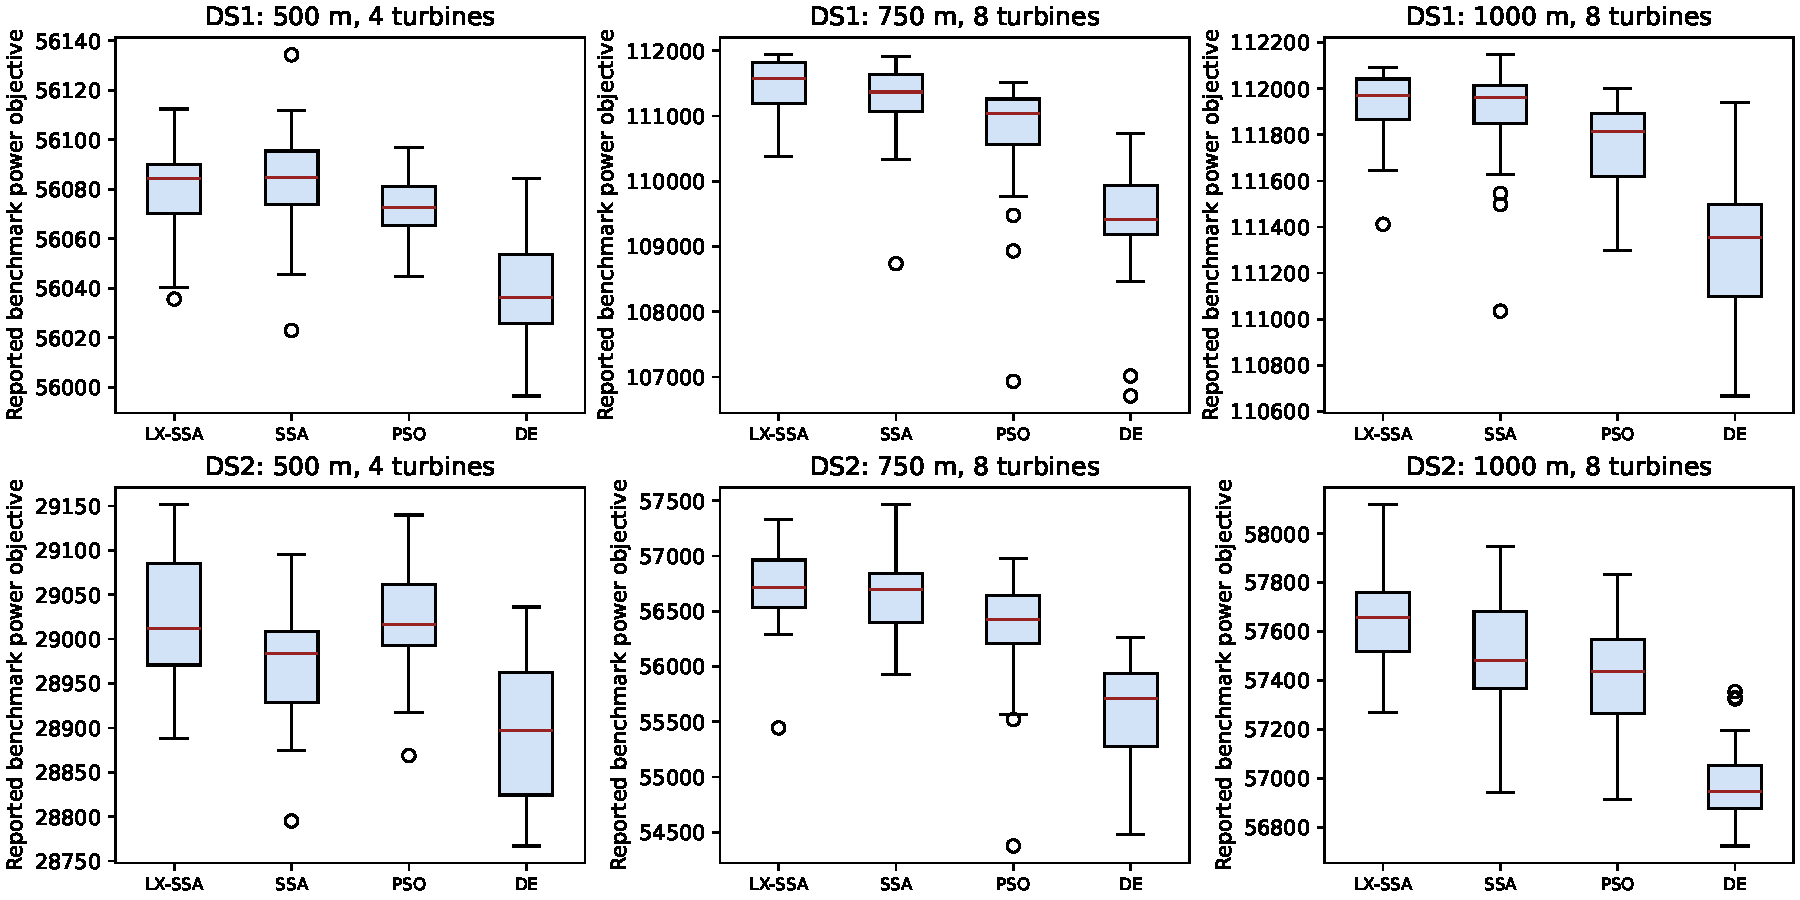
\includegraphics[width=\textwidth]{selected_power_boxplots.pdf}
\caption{Run-level distributions of the reported power objective in the six selected follow-up cases. Each box contains 30 runs. Comparisons are descriptive because LX-SSA has twice as many recorded objective evaluations as the other algorithms.}
\label{fig:selected-boxplots}
\end{figure*}

In the reported final-solution data, LX-SSA used 6,030 objective evaluations per run; SSA, PSO and DE each used 3,030. The common iteration cap (100) therefore did \emph{not} produce an equal objective-evaluation budget. Table~\ref{tab:followup-results} and Fig.~\ref{fig:selected-boxplots} describe performance at these \emph{different budgets}; neither should be read as evidence of better performance at equal computational cost. The repeated runtime field contains a single batch-level measurement divided by 30 for each algorithm/case, not 30 independent timings. Because the hardware and software environment are undocumented, we do not conduct runtime hypothesis tests or claim a measured speed advantage.

The distributions were tested using an independent-sample Kruskal--Wallis test within each case, followed by two-sided Mann--Whitney tests comparing LX-SSA with each of SSA, PSO and DE; the three comparisons \emph{within each case} were adjusted by Holm's procedure. Positive mean differences and positive rank-biserial effects favor LX-SSA on the reported power objective. The seed labels alone do not establish matched initial conditions or paired random streams, so a paired signed-rank test is not justified. These tests describe differences in the \emph{recorded unequal-budget runs}; they do not remove the evaluation-budget confounding. We do not use the workbooks' all-algorithm Friedman/Wilcoxon summaries, which involve additional algorithms and assume a pairing that the supplied metadata do not establish.

\begin{table*}[!t]
\centering\caption{Exploratory independent-sample tests for the selected follow-up cases. $H$ and $p_{\rm KW}$ are the four-algorithm Kruskal--Wallis statistic and $p$ value. The three adjusted $p$ values compare LX-SSA with each baseline using Mann--Whitney tests with Holm correction within the case. Additional numerical precision for the $p$ values is provided in the accompanying analysis CSV; these are conventional test $p$ values, not exact enumeration.}
\label{tab:exploratory-tests}
\footnotesize\setlength{\tabcolsep}{3pt}
\begin{tabular}{ccccccccc}
\toprule
DS & Radius (m) & $N$ & $H$ & $p_{\rm KW}$ & Baseline & $\Delta$ power & $p_{\rm Holm}$ & Rank-biserial \\
\midrule
1 & 500 & 4 & 52.21 & 2.697e-11 & SSA & -2.06 & 0.6735 & -0.06 \\
1 & 500 & 4 & 52.21 & 2.697e-11 & PSO & +7.17 & 0.09029 & +0.30 \\
1 & 500 & 4 & 52.21 & 2.697e-11 & DE & +42.80 & 4.288e-08 & +0.85 \\
\midrule
1 & 750 & 8 & 67.42 & 1.525e-14 & SSA & +164.45 & 0.2398 & +0.18 \\
1 & 750 & 8 & 67.42 & 1.525e-14 & PSO & +721.60 & 7.661e-05 & +0.62 \\
1 & 750 & 8 & 67.42 & 1.525e-14 & DE & +2032.33 & 1.493e-10 & +0.99 \\
\midrule
1 & 1000 & 8 & 61.68 & 2.574e-13 & SSA & +41.08 & 0.5895 & +0.08 \\
1 & 1000 & 8 & 61.68 & 2.574e-13 & PSO & +182.87 & 8.706e-05 & +0.62 \\
1 & 1000 & 8 & 61.68 & 2.574e-13 & DE & +593.41 & 2.43e-09 & +0.92 \\
\midrule
2 & 500 & 4 & 38.23 & 2.528e-08 & SSA & +52.72 & 0.03391 & +0.36 \\
2 & 500 & 4 & 38.23 & 2.528e-08 & PSO & +0.90 & 0.8303 & -0.03 \\
2 & 500 & 4 & 38.23 & 2.528e-08 & DE & +127.20 & 6.462e-06 & +0.71 \\
\midrule
2 & 750 & 8 & 63.06 & 1.305e-13 & SSA & +87.89 & 0.3042 & +0.16 \\
2 & 750 & 8 & 63.06 & 1.305e-13 & PSO & +382.94 & 0.001175 & +0.52 \\
2 & 750 & 8 & 63.06 & 1.305e-13 & DE & +1141.03 & 5.87e-10 & +0.96 \\
\midrule
2 & 1000 & 8 & 66.62 & 2.258e-14 & SSA & +154.65 & 0.01988 & +0.35 \\
2 & 1000 & 8 & 66.62 & 2.258e-14 & PSO & +263.01 & 8.168e-05 & +0.62 \\
2 & 1000 & 8 & 66.62 & 2.258e-14 & DE & +675.68 & 1.648e-10 & +0.99 \\

\bottomrule
\end{tabular}
\end{table*}

The selected results show a mixed mechanism-level comparison. For Dataset~I at 500~m/4, SSA exceeds LX-SSA by 2.06 objective units in sample mean and the Holm-adjusted comparison does not distinguish their run distributions ($p=0.6735$). At 750~m/8, the LX-SSA mean exceeds SSA by 164.45 and 87.89 units for Datasets~I and II, respectively, while neither SSA comparison survives the within-case Holm adjustment ($p=0.2398$ and $p=0.3042$). Dataset~II at 1000~m/8 shows a higher LX-SSA mean than SSA by 154.65 units ($p_{\mathrm{Holm}}=0.01988$); this difference remains confounded by LX-SSA's larger evaluation budget. The larger observed differences against DE and PSO cannot establish relative efficiency under equal computational effort.

These post hoc, unequal-budget tests are a limited diagnostic, not a basis for a universal superiority claim. In more crowded cases, the workbooks contain infeasible layouts with penalty-scale values in the \texttt{WakeLoss} column; reporting those raw means as physical wake deficits would be misleading. Equal-budget reruns, documented matched-seed initialization, feasibility-rate reporting for every case, and a verified objective definition are needed before the additional data can replace the historical tables or support definitive comparative claims.
